\documentclass[a4paper,11pt]{book}
\usepackage[utf8]{inputenc}
\usepackage{graphicx}
\usepackage{cancel}
\usepackage{emptypage}
\usepackage{subcaption}
\usepackage{hyperref}
\usepackage{url}
\usepackage{mathrsfs}
\usepackage{amsmath}
\usepackage{amsfonts}
\usepackage{ amssymb }
\usepackage{mathcomp}
\usepackage{gensymb}
\usepackage{tensor}
\usepackage{tcolorbox}
\usepackage{lmodern}
\usepackage{wasysym}
\usepackage{enumerate}
\setlength{\parindent}{2.0em}
\setlength{\parskip}{0.6em}
\renewcommand{\baselinestretch}{1.25}

%\usepackage{tgschola}

\usepackage{geometry}
\geometry{
	a4paper,
	total={170mm,257mm},
	left=35mm,
	right=35mm,
	top=25mm,
}

\begin{document}

\author{Sergio Lobo}
\title{Draft: Calibration of DESI resdshift data using ML}
\date{\today}

\frontmatter
\begin{titlepage}
    \begin{center}
        \vspace*{0.8 cm}
        
        \Large
        \textbf{Draft: Calibration of DESI readsfiht measurements using machine learning}
        
       by\\
        \large
        
        
        \vspace{1.0cm}
        
        \textbf{Sergio David Lobo Bolaño}
        
        \vspace{1.1 cm}
        \large
        Undergraduate Monograph \\
                \vspace{1cm}
        \normalsize 
        Submitted to the Department of Physics\\
         in fulfillment of the requirements for\\
       the degree of\\
       \vspace{0.4 cm}
       \LARGE
       Bachelor of Science in Physics\\
      
        \vspace{1cm}
        
        \normalsize
        Advisor\\
        \Large
        Jaime Ernesto Forero-Romero
        
        

\begin{center}

\includegraphics[width=0.4\linewidth]{TeX_files/universidaddelosandes}
\end{center}

                \vspace{2cm}
        \normalsize
        Department of Physics	\\
        UNIVERSIDAD DE LOS ANDES\\
        COLOMBIA\\
        \today
        
    \end{center}
\end{titlepage}
\tableofcontents
\listoffigures
\listoftables
\mainmatter
\chapter*{\centering \begin{normalsize}Abstract\end{normalsize}}
\begin{quotation}
	\noindent The DESI (Dark Energy Spectroscopic Instrument) project will conduct a five-year survey designed to cover 14.000 $deg^2$ by studying baryon acoustic oscillations (BAO) and redshift-space distortions (RSD). DESI needs simulations for its design, development, and operation, it uses simulations to evaluate the data pipelines and measurements of redshifts from the spectrometers. In particular, DESI uses a simulated survey of mock galaxies to compare their redshifts with the -also simulated- redshift measurements of DESI. These redshift measurements, however, present differences with respect to the true redshifts values of the mock galaxies. It is necessary to correct these measurements so that the instrument can work properly when tested in the real world. 
	
	The objective of this monograph is, therefore, to apply machine learning (ML) methods to the simulation data to recover the true redshift measurements of the Bright Galaxy Sample using observational variables as input. 
	
	First, we pre-process the data and select the variables as input for the ML models, this variables are the fluxes from the different observation bands, which are the $g, r, z, WISE 1,$ and $WISE 2$ bands, as well as the redshift output of the instrument's pipeline. The true redshift from the mock galaxies is used as output. We train and test support vector regression (SVR) and kernel ridge regression (KRR) models using cross-validation and grid search, later we use an ensemble model of different KRRs, this results in the best model with a coefficient of determination, $r^2 = 0.98$. This could be used to improve the accuracy of DESI when working in the five-year survey. Future work can be done in the fine-tunning of the model hyper-parameters, trial of other model classes and different data preprocessing methods, as well as the application of this results to different classes of targets in the survey.   
\end{quotation}
\clearpage
\chapter{Introduction}

TODO Introduction and motivation of the project.

\section{Objectives}

\subsection{General Objective}
\begin{itemize}
	\item Determine the relation between the redshift simulated mesurements by DESI   and the intrinsic (simulated) redshift of BGS galaxies, to calibrate the instrument for real-world use using kernel method of machine learning
\end{itemize}

\subsection{Specific Objective}
\begin{itemize}
	\item Characterize the dataset using a simple statistical and graphical procedure to select the set of meaningful features as input to the machine learning algorithms. 
	\item Determine the set of computational parameters such as memory requirement, number of processors per node and size of dataset that performs the best on the cluster of the university restricted to constraints of resources, execution time and waiting time in queue.
	\item Train and adjust the hyper-parameter of the models by using grid-search and cross validation.
	\item Select the best model based on performance on unseen data and model simplicity.
\end{itemize}

\section{Context}
TODO Important concepts and definition from the DESI project and Machine learning
\subsection{DESI Project}
TODO Description of the Desi project and instrument, how the results are simulated. 
\subsection{Machine Learning}
TODO Supervised Learning, regression and classification, principal method of ML:
\subsubsection{Kernel Methods}
TODO Introduction, mathematics, and parameters of the model. 
\subsubsection{Neural Networks}
TODO Introduction, mathematics, and parameters of the model. 

conclusions about the complexity of the neural networks. 

\chapter{Methodology}
\section{Introduction}
This chapter explain the procedure to achieve the objectives declared in the previous chapter. Each objective consist of a series of activities that produce an outcome, each one contributing to reach the general objective of this monograph. First, a description of the data pre-processing, then the selection of computer parameters and finally, a description of the methodology for training and testing the models. 
\section{Data analysis and pre-processing}
The dataset consists of two files, one with the redshift measurement of DESI (TAR file) and the other with simulated true redshifts (TRUTH file). Apart from this, the files also contain several variables related to the simulations parameters, the type of target, the observation conditions, etc. 
\begin{figure}[h!]
	\centering
	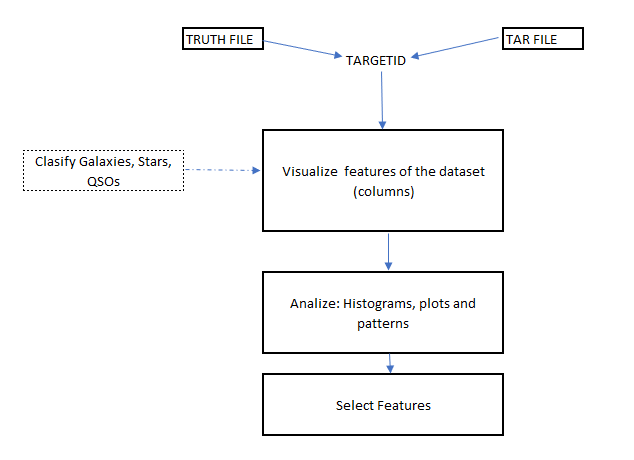
\includegraphics[width=1\linewidth]{TeX_files/Imagenes/metho_1}
	\caption{General methodology to understand the dataset and extract valuable features.}
	\label{fig:metho1}
\end{figure}
Figure \ref{fig:metho1} shows the general step-by-step method to understand the data. In the first step, the two files have to be linked by the variable TARGETID, this variable represent the identity of a target through the whole pipeline of the experiments (observation and measurements). After this, the next step is to discriminate by target type and observe the behavior of the other variables in the files. From this one can neglect some basic variables that give no relevant information to the problem. A second analysis can be executed with more details, to see if the variables hold any relation with the redshift measurement, using histograms and approximating distribution. This is done to select which variables (or features) can be used to explain the difference between the true redshift of a galaxy and the redshift measured by DESI. The details of this can be found in Chapter \ref{Ch:Data}. After the features are selected, they will be scaled so that the means are equal to zero and the variance to one. 

\section{High performance computing analysis}

The training time if the model depends on the size of the training set, however, since it is going to be executed in parallel in the computing cluster of the University, the training time will also depend on the resources of the hardware. For example, the memory of the machine and the number of processor in which the code will be parallelized, as well as the number of processor that the computer (or node) actually has. To see what is the best combination of parameters to train the models in a reasonable amount of time up to a reasonable accuracy, it will be necessary to restrict also the size of the dataset used for training.

\begin{figure}[h!]
	\centering
	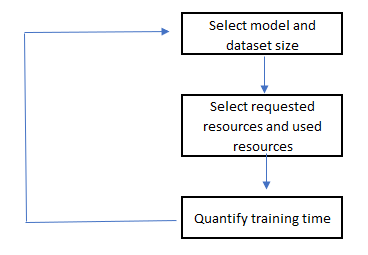
\includegraphics[width=0.7\linewidth]{TeX_files/Imagenes/metho_2}
	\caption{Sequence of step to gather enough information to understend the relation between computation time, memory, dataset size and processors.}
	\label{fig:metho2}
\end{figure}

Figure \ref{fig:metho2} shows the step to accomplish this. First, select the model and architecture (grid search / cross validation, explained next) and the dataset size, in order to see how the training time scales with size, it is necessary to select different sizes, in this case, 100, 1000, 5000, and 10000. Then, the algorithm have to be run in certain number of processors, and with certain RAM memory,in this case, we will try 1, 4, 8 and 16 processors, and 16, 32, 64 and 128 GB of memory. The expected result is number of parameters to run the complete training algorithm on a big dataset. 
\section{Machine Learning}
Once we understand the scalability of the training time with respect to hardware variables, it is time to train and test the models. For this the dataset will be divided in a training set, corresponding to 75\% of the dataset and a test set (the rest 25 \%) as shown in Figure \ref{fig:metho3}. After this, according to the results of the previous section, the training set will be split in subsets of specific size, this subsets will be again divided into a development and evaluation sets, to apply to them the grid search and cross validation. This two methods are used to select the hyper-parameters of the models and to quantify the error of the algorithms. 
\begin{figure}[h!]
	\centering
	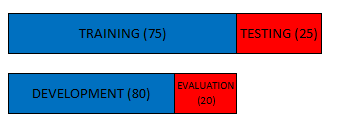
\includegraphics[width=0.6\linewidth]{TeX_files/Imagenes/metho_3}
	\caption{Divition of the dataset in train and test. The train set is divided in development-evaluation subsets.}
	\label{fig:metho3}
\end{figure}
\subsection{Training}
For training, we will use grid search and cross validation to select the hyper-parameters of the models.
The grid search method correspond to train the model with different combinations of parameters as in going over a grid, and search for the combinations of parameters that give the best results. This is used alongside cross validation, which consist on training the model several times by randomly assigning the development and the evaluation sets. Therefore, it reports the mean and standard error of the metrics of the trained models.
\subsection{Testing}
Once the models are trained, they will be test on the unseen 25\% of the data to check its generalization ability. This means, that we need to see whether the model truly 'learns' to predict redshifts or just memorized the training dataset. To select the best performing algorithm on the test dataset, the criterion will be the $r^2$ measure and the simplicity of the model.



In general, the methodology for this project consist in analysing the complete dataset and selecting the valuable features than can be used to predict a correct redshift, finding the scalability of the training time with respect to the size of the dataset and the cluster resources, an finally, training an evaluating the machine learning models. 





\chapter{Data}
\label{Ch:Data}

\section{Introduction}


\section{Data descripcion}

The dataset used consist of two FITS files corresponding to the simulated observations of the DESI instrument and the "truth" data from cosmological simulations. Each data file has a key column called TARGETID, this variables is the same across all simulations and identifies a particular object in the sky, thus it is needed to relate both datasets. 
\subsection{Simulated expected results - truth file}
This file contains the data from the cosmological simulation of the target objects. Thus, this file contains the expected redshift that the instrument \textit{should} measure. The complete list of columns in the file is shown in table \ref{tab:true_car}\footnote{Additional information on \url{https://desidatamodel.readthedocs.io/en/stable/}}. Since we aim to correct the measurements of redshifts given by the instrument, the variable TRUEZ will be our target variable or "\textit{output}" to the machine learning models. The rest of the information will be used mostly for understanding the dataset but no as part of the ML model, since this information would not be available to the instrument in reality. This dataset contains the redshift of 24.851.543 objects. 
\begin{table}[!htbp]
	\centering
	\begin{tabular}{c}
		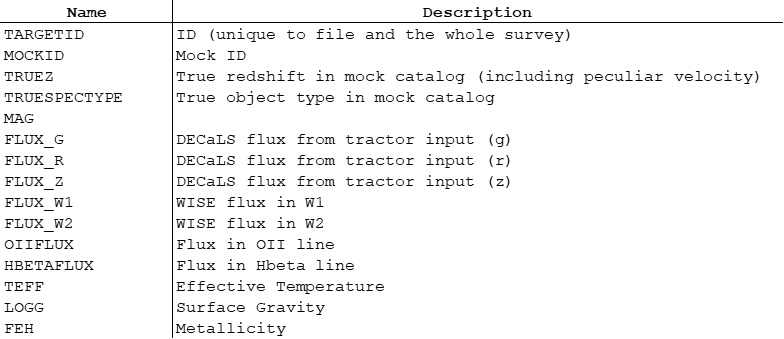
\includegraphics[width=0.9\linewidth]{TeX_files/Imagenes/Imagen2}
	\end{tabular} 
	\caption{Columns in the cosmological simulation data file}
	\label{tab:true_car}
\end{table}
\subsection{Simulated Observations - target file}
This file contains the redshift values of the targets as measured by the instrument in simulation. Apart from this, it also contains the columns shown in table \ref{tab:tar_car}. The different characteristics listed in Table \ref{tab:tar_car} are the ones that we will use as input in our machine learning models, since is the data available from the instrument. This dataset contains the redshift of 2.131.896 objects. 
\begin{table}[!htbp]
	\centering
	\begin{tabular}{c}
	    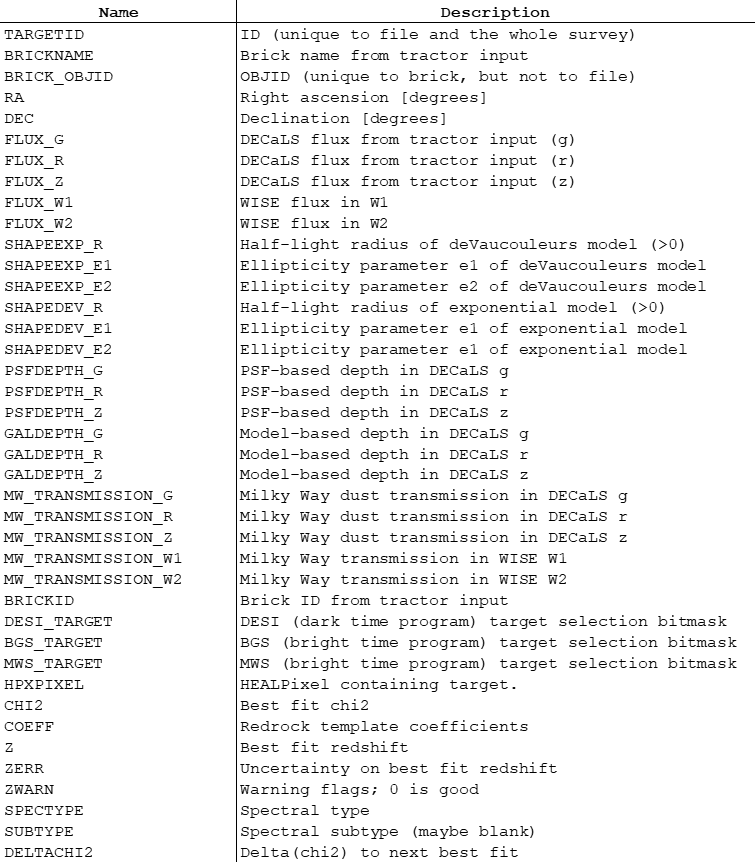
\includegraphics[width=0.9\linewidth]{TeX_files/Imagenes/Imagen1}	
	\end{tabular} 
	\caption{Columns in the Simulated Observations data file }
	\label{tab:tar_car}
\end{table}
Since the files don´t have the same amount of points, they were cut to the one with the least (the target file) by linking the rows by its TARGETID. 
\section{Overview of the dataset}
\subsection{Redshift relations}
To understand the dataset, the first thing we need to do is see how the Z and TRUEZ variables behave. In Figure \ref{fig:z-truez} we see three distinct regions: a 45-degree line that correspond to the redshifts measurements of DESI that are very close to the expected 'real' value, a square region where the data seems to scatter randomly except for some line groupings, and a third region of horizontal line near True Z = 0. The task is therefore to dissolve the square region and have all the points along the diagonal line.   
\begin{figure}[h!]
	\centering
	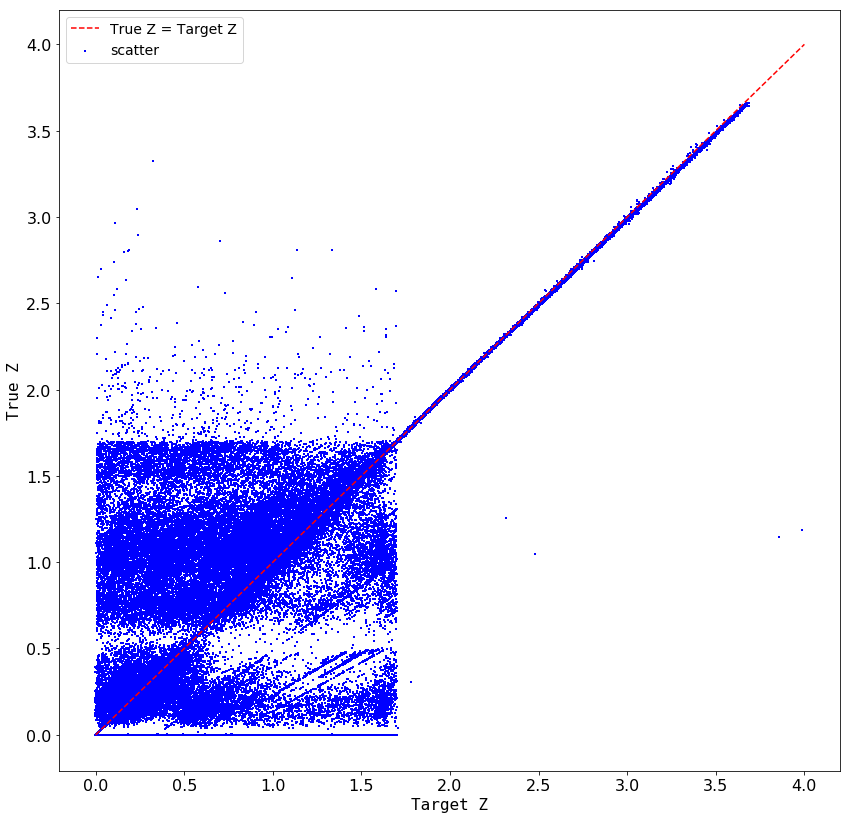
\includegraphics[width=1.0\linewidth]{TeX_files/Imagenes/z-truez}
	\caption{Relation between the 'observed' readshift - target Z, and the 'generated' redshift - True Z.}
	\label{fig:z-truez}
\end{figure}

Now, cutting along the MAG (magnitude) variable, it is possible to see the distribution of magnitudes of the gathered data an see if there is any relation with the square region. Figure \ref{fig:mag-dist} shows this distribution and Figure \ref{fig:mag-prop-dist} shows the fraction redshifts of each bin that is within a 1\% error of the true value. We can see that the majority of the redshift is near its true value, however some valleys indicate that some regions (for example between 15 and 17 in magnitude) are not that good. For simplicity, from now on we will refer to the \textbf{simulated expected redshift} as TRUEZ (the output to the ML models) and the \textbf{simulated observations of the targets} as Z (the input to the models) or TARZ.
\begin{figure}
	\centering
	\begin{subfigure}[b]{1.0\textwidth}
		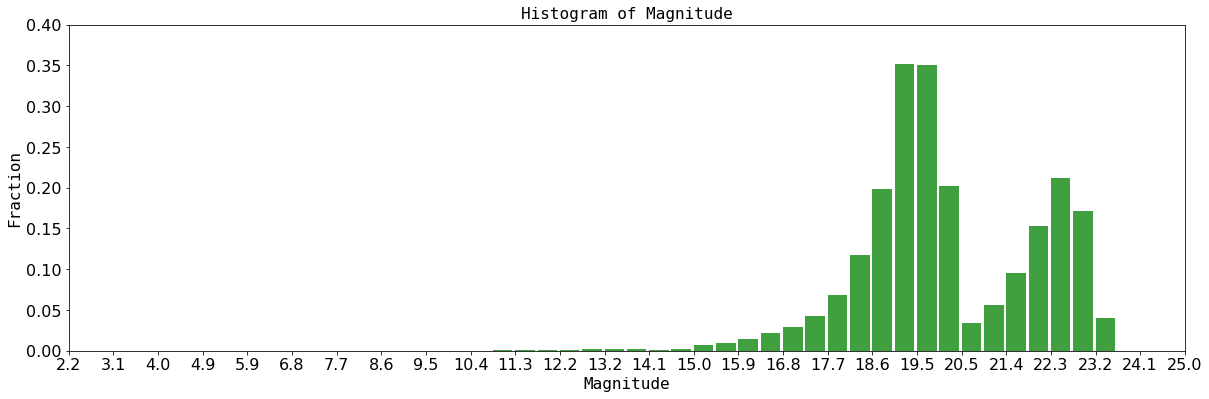
\includegraphics[width=1\linewidth]{TeX_files/Imagenes/mag-dist}
		\caption{}
		\label{fig:mag-dist} 
	\end{subfigure}	
	\begin{subfigure}[b]{1.0\textwidth}
		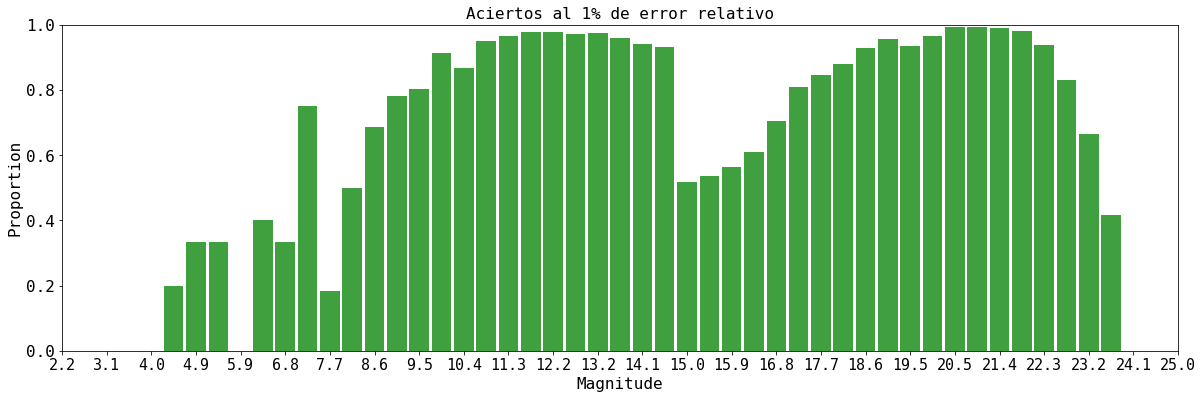
\includegraphics[width=1\linewidth]{TeX_files/Imagenes/mag-prop-dist}
		\caption{}
		\label{fig:mag-prop-dist}
	\end{subfigure}
	\caption{(a) Distribution of magnitudes in the dataset. (b) Proportion of the number of measured redshifts that are within the 1\% error of their corresponding TRUEZ }
	\label{fig:mag-dist-both}
\end{figure}
\subsection{Spectral types}
From figure \ref{fig:mag-dist-both} it is possible to infer that the different magnitudes of the targets can be related to the different regions on figure \ref{fig:z-truez}, and this difference in magnitude is also related to the SPECTYPE of each target. The spectral type of the data in the tar-file is distributed as shown in Table \ref{tab:espectype-N}. Near 85\% of the dataset is composed of Galaxy-type objects, for this reason, this is the most interesting class.
\begin{table}[!h]
	\centering
\begin{tabular}{c|c|c}

	SPECTYPE & N samples & \% of dataset \\ 
	\hline 
	Galaxy & 1796213 & 84.25 \\ 

	QSO & 194319 & 9.11 \\ 

	Star & 141364 & 6.63 \\ 

	Total & 2131896 & 100 \\ 

\end{tabular} 
\caption{Spectral type distribution of the tar file. }
\label{tab:espectype-N}
\end{table}
\begin{figure}
	\centering
	\begin{subfigure}[b]{0.5\textwidth}
		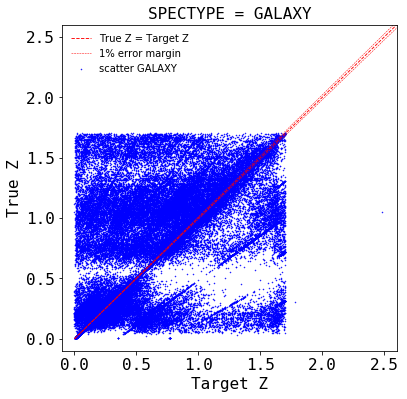
\includegraphics[width=1\linewidth]{TeX_files/Imagenes/GALAXY-z-truez}
		\caption{}
		\label{fig:GALAXY-z-truez} 
	\end{subfigure}	
	\begin{subfigure}[b]{0.5\textwidth}
		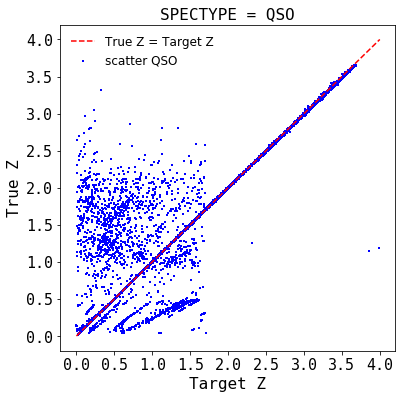
\includegraphics[width=1\linewidth]{TeX_files/Imagenes/QSO-z-truez}
		\caption{}
		\label{fig:QSO-z-truez}
	\end{subfigure}
	\begin{subfigure}[b]{0.5\textwidth}
	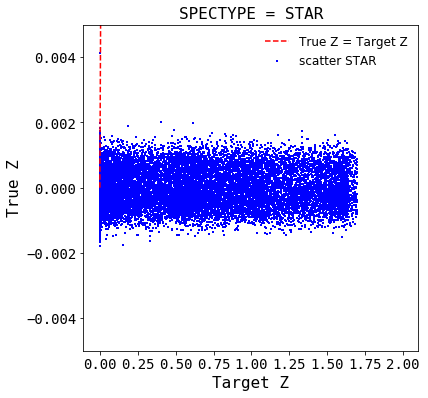
\includegraphics[width=1\linewidth]{TeX_files/Imagenes/STAR-z-truez}
	\caption{}
	\label{fig:STAR-z-truez}
	\end{subfigure}
	\caption{ Redshift relation for (a) Galaxy-type objects, (b) QSO-type objects, and (c) Star-type objects }
	\label{fig:SPECTYPE-z-truez}
\end{figure}

The redshift relations similar to Figure \ref{fig:z-truez} discriminated by SPECTYPE are shown in Figure \ref{fig:SPECTYPE-z-truez}, where the three regions in Figure \ref{fig:z-truez} seems to be related to each spectral type. The GALAXY objects are distributed along a square and there are lines formed at angles different than 45, which means that there is a relation between the two variable but 'out of calibration'. It is worth mentioning that Figure \ref{fig:GALAXY-z-truez}  can be deceiving, because 96.34\% of the Galaxy-type data is within the 1\% margin line in the figure, which means that the square is formed only by the 3.66 \% of the galaxy data, corresponding to approximately  65.742 measurements, still a lot. 

The QSO-type objects in Figure \ref{fig:QSO-z-truez} correspond to the 45-degree line in Figure \ref{fig:z-truez} since the majority of points are along this line, although the same line patter and dispersion of the galaxy-type objects are present, but in least quantity. However, the Star-type in Figure \ref{fig:STAR-z-truez} is randomly scattered over the TARZ range and correspond to the horizontal line in Figure \ref{fig:z-truez}. Once again, the most interesting SPECTYPE is GALAXY, because it has the majority of error in TARZ, and also presents different patterns, QSO are already fine and are not a priority while STAR is completely random a represent a small fraction of the whole dataset. From now on we will focus on Galaxy-type objects only.  

\subsection{Galaxy-type objects}
Galaxy-type objects are clasified as Bright Galaxy Survey (BGS), Emission Line Galaxies (ELG) and Luminous Red Glaxies (LRG) distributing according to Table \ref{tab:Galaxy-sub-types}. In this case, the sub-types are more evenly distributed. The redshift relations of each sub-type is shown in Figure \ref{fig:GALAXY-SUB-z-truez}. BGS and ELG follow similar pattern, however ELG is more disperse while BGS is clustered along the TARZ = TRUEZ line, whereas LRG sub-type is already perfect. 
\begin{table}[!h]
\centering
\begin{tabular}{c|c|c}
	Galaxy subtype & N samples  & \% of dataset  \\ 
	\hline 
	BGS & 889336 & 49.51 \\ 	 
	ELG & 601847 & 33.51 \\  
	LRG & 305030 & 16.98 \\ 
	Total & 1796213 & 100 \\  
\end{tabular} 
\caption{Distribution of Galaxy sub-types}
\label{tab:Galaxy-sub-types}
\end{table}

Note that the line structures are more visible in Figure \ref{fig:BGS-z-truez} than in Figure \ref{fig:ELG-z-truez}, therefore, to extract the relevant features in the tar dataset that may be related to this structure, we will use the BGS subset and then see if the feature extracted are also useful for the ELG subset. Therefore, from now on we will use only the BGS data subset and proceed to find the relevant features (in Table \ref{tab:tar_car})

\begin{figure}[!htbp]
	\centering
	\begin{subfigure}[b]{0.5\textwidth}
		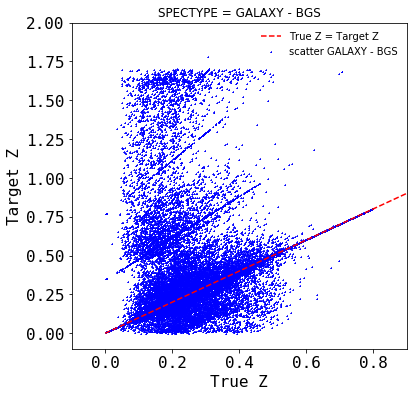
\includegraphics[width=1\linewidth]{TeX_files/Imagenes/BGS-z-truez}
		\caption{}
		\label{fig:BGS-z-truez} 
	\end{subfigure}	
	\begin{subfigure}[b]{0.5\textwidth}
		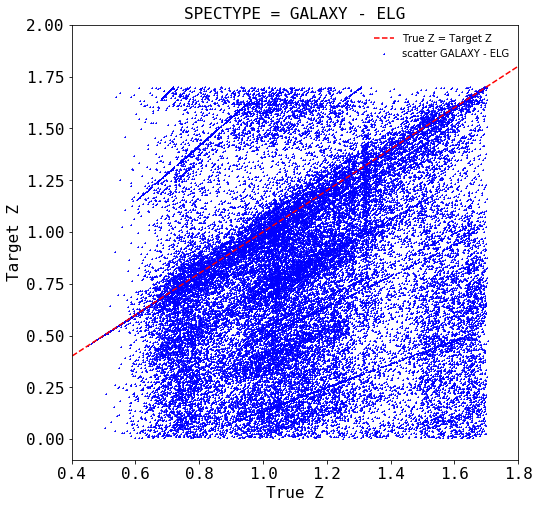
\includegraphics[width=1\linewidth]{TeX_files/Imagenes/ELG-z-truez}
		\caption{}
		\label{fig:ELG-z-truez}
	\end{subfigure}
	\begin{subfigure}[b]{0.5\textwidth}
		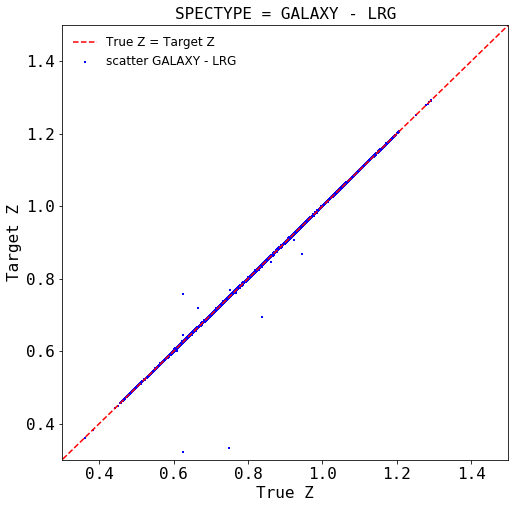
\includegraphics[width=1\linewidth]{TeX_files/Imagenes/LRG-z-truez}
		\caption{}
		\label{fig:LRG-z-truez}
	\end{subfigure}
	\caption{ Redshift relation for Galaxy (a) BGS-type objects, (b) ELG-type objects, and (c) LRG-type objects }
	\label{fig:GALAXY-SUB-z-truez}
\end{figure}

\section{Relevant Features}
The ability of the instrument for measuring the correct redshift will probably depend on the quality of the fluxes that the fiber optics receive. The fluxes of the objects are related to its magnitude, as we saw en Figure \ref{fig:mag-dist-both}, magnitude is related to the correct prediction of the instrument's Z, but since the information of magnitude is known to instrument in form of fluxes, this variables will be explored next. The six fluxes variables are named in Table \ref{tab:tar_car}.  The distributions of the fluxes in the BGS dataset are shown in Figure \ref{fig:bgs-flux-dist}.

\begin{figure}[h!]
	\centering
	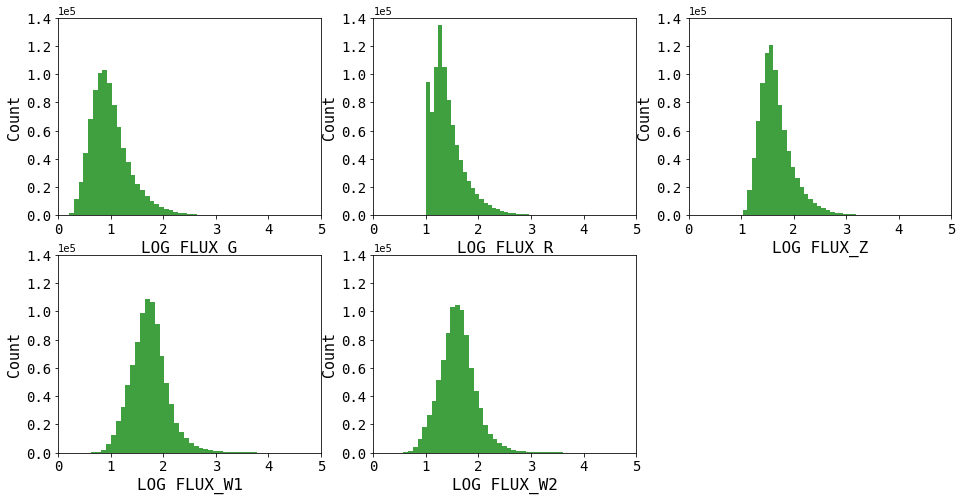
\includegraphics[width=1\linewidth]{TeX_files/Imagenes/BGS-flux-dist}
	\caption{Distribution of the flux variable in the BGS subset.}
	\label{fig:bgs-flux-dist}
\end{figure}

In order to keep track of the relation between TARZ y TRUEZ and see the behavior of the flux variable with respect to the two, we define the following variable
\begin{equation}
	\alpha = \frac{TRUEZ}{TARZ},
\end{equation}
therefore, alpha have a value near 1 when the redshifts are along de 45-degree line. 
\begin{figure}[!htp]
	\centering
	\begin{subfigure}[t]{0.5\textwidth}
		\centering
		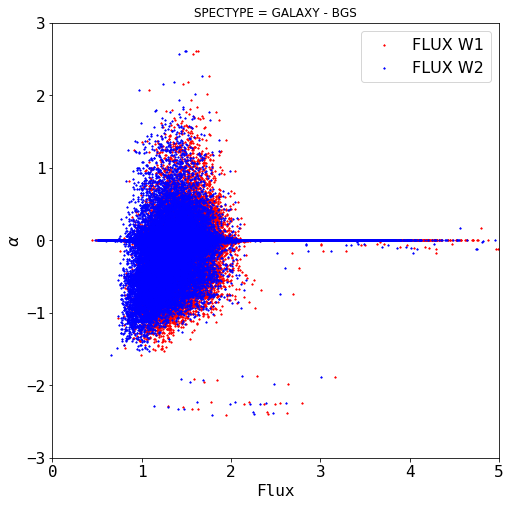
\includegraphics[height=3in]{TeX_files/Imagenes/BGS-FLUXW-ALPHA}
		\caption{}
	\end{subfigure}%
	\begin{subfigure}[t]{0.5\textwidth}
		\centering
		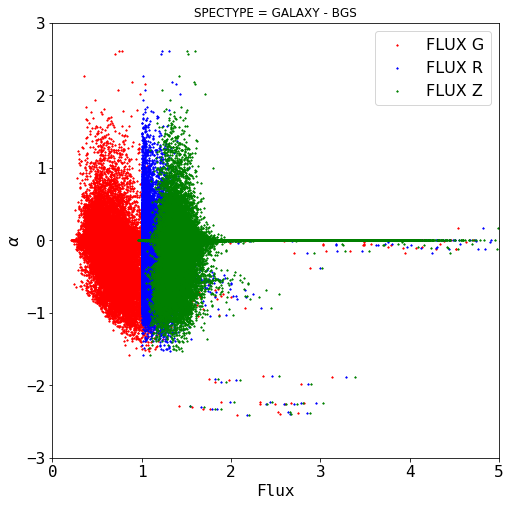
\includegraphics[height=3in]{TeX_files/Imagenes/BGS-FLUXRGZ-ALPHA}
		\caption{}
	\end{subfigure}
	\caption{Relation between fluxes, TRUEZ and TARZ. (a) $\alpha$ as a function of W1 and W2 fluxes. (b)$\alpha$ as a function of G, R and Z fluxes }
\end{figure} 
\chapter{Results}

\section{Scalability of the training time of the ML models} %High performance computing (HPC) results}

Since the BGS dataset contains about 800000 data points, the training of algorithms, model selection and validation can be too demanding, in processing and memory. Therefore, it is necessary to evaluate how the training time scales with the data when running in the High Performance Computing (HPC) cluster of the University, taking account several variables as the number of processor to run in parallel the algorithm and the resources requested to the cluster. In particular, we will focus on the following variables:
\begin{align*}
m &= \text{Requested memory to solve the job [Gb]},\\
n_{jobs} &= \text{Number of jobs to run in parallel},\\
ppn &= \text{Requested proccesors per node},\\
n &= \text{size of the dataset used},\\
M &= \frac{n_{jobs} \times n}{ppn \times m}.
\end{align*}
\begin{figure}[ht!]
	\centering
	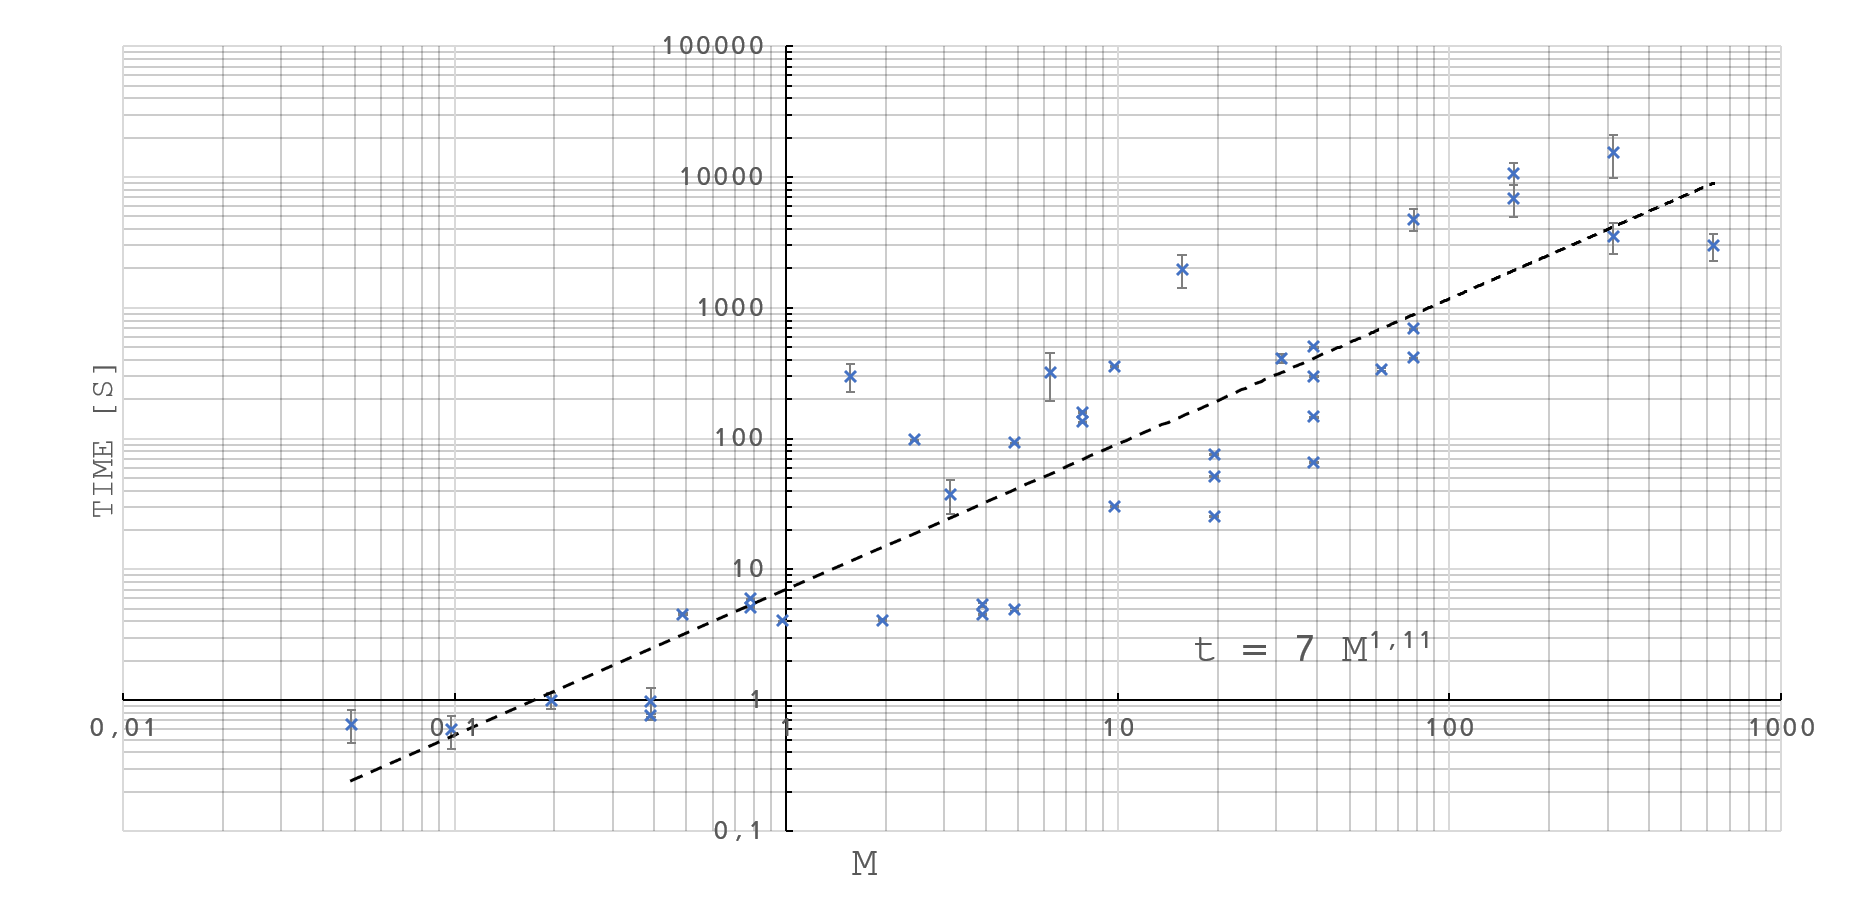
\includegraphics[width=1.0\linewidth]{TeX_files/Imagenes/hpc_results}
	\caption{Time as a function of requested memory, number of data points and jobs used to train the model.}
	\label{fig:hpcresults}
\end{figure}

The variable $M$ measures the relation between the requested resources and the used. Figure \ref{fig:hpcresults} shows how time increases as a function of variable M. Note that $M^{-1}$ can be seen as a 'unitary memory', that is, the memory used per data per processor,
\begin{equation*}
M^{-1} = \frac{m}{p_u \times n},
\end{equation*}
where $p_u = n_{jobs}/ppn$ is the fraction of the requested processors that is actually being used by the parallel code. Therefore, when $M$ is big, it means that there is too much data per memory per processor, and the time to train the model is to high. It is worth mentioning that the time were measure for the kernel ridge regression model particularly, using grid search and 3-fold cross validation. Others model may be faster or slower to train, but the behavior should be the same. The time of training for a given $M$ can be aproximated by the relation
\begin{equation}
	t = 7M^{1.11} [s].
\end{equation}

This results have to be constrained to the waiting time in queue of the cluster, in general, the smaller M, the best time, but that means, using small dataset or increasing the resources, but for the second option, the more resources you request, the longer the queue and waiting time to execute the code. It was fond that a configuration with \textbf{$n_{jobs} = 16$, $ppn = 32$, $m = 128 Gb$ and $n = 100000$}, gives good results. n is critical since it determines how well the model will learn, 100000 data points works very well as it will be shown in the next sections.  

\section{Model results}

The three model tested consist of a KRR, a SVR and an ensemble model. The original BGS dataset was divided into a 75 - 25 train-test set, from the 75 \%, each model was trained on a subset of size 100.000, as mentioned in the previous section. To account for the bias, the same model was trained in tree 100.000 dataset and the results were averaged. The selection of the model hyperparameters was made by using grid search a 3-fold cross validation, using a 80-20 development-evaluation scheme. 

\subsection{Support Vector Regression (SVR) Model}

The grid-search and cross-validation on the train-development set use the $r^2$ measure to select the best parameters. 

\begin{verbatim}
--------------------------------------------------------------------------
Model 1:
Best parameters set found on development set:

{'gamma': 0.1, 'C': 1, 'kernel': 'rbf'}

Grid scores on development set:

0.877 (+/-0.001) for {'gamma': 0.001, 'C': 1, 'kernel': 'rbf'}
0.927 (+/-0.011) for {'gamma': 0.1, 'C': 1, 'kernel': 'rbf'}
0.848 (+/-0.017) for {'gamma': 1, 'C': 1, 'kernel': 'rbf'}
0.896 (+/-0.001) for {'gamma': 0.001, 'C': 10, 'kernel': 'rbf'}
0.924 (+/-0.010) for {'gamma': 0.1, 'C': 10, 'kernel': 'rbf'}
0.870 (+/-0.013) for {'gamma': 1, 'C': 10, 'kernel': 'rbf'}
0.898 (+/-0.006) for {'gamma': 0.001, 'C': 100, 'kernel': 'rbf'}
0.922 (+/-0.007) for {'gamma': 0.1, 'C': 100, 'kernel': 'rbf'}
0.868 (+/-0.020) for {'gamma': 1, 'C': 100, 'kernel': 'rbf'}

r2 score computed on the full evaluation set:

0.928

--------------------------------------------------------------------------
Model 2:

Best parameters set found on development set:

{'gamma': 0.1, 'C': 1, 'kernel': 'rbf'}

Grid scores on development set:

0.878 (+/-0.002) for {'gamma': 0.001, 'C': 1, 'kernel': 'rbf'}
0.928 (+/-0.007) for {'gamma': 0.1, 'C': 1, 'kernel': 'rbf'}
0.859 (+/-0.020) for {'gamma': 1, 'C': 1, 'kernel': 'rbf'}
0.892 (+/-0.002) for {'gamma': 0.001, 'C': 10, 'kernel': 'rbf'}
0.919 (+/-0.019) for {'gamma': 0.1, 'C': 10, 'kernel': 'rbf'}
0.859 (+/-0.010) for {'gamma': 1, 'C': 10, 'kernel': 'rbf'}
0.902 (+/-0.003) for {'gamma': 0.001, 'C': 100, 'kernel': 'rbf'}
0.909 (+/-0.006) for {'gamma': 0.1, 'C': 100, 'kernel': 'rbf'}
0.861 (+/-0.020) for {'gamma': 1, 'C': 100, 'kernel': 'rbf'}

r2 score computed on the full evaluation set:

0.92
--------------------------------------------------------------------------
Model 3:

Best parameters set found on development set:

{'gamma': 0.1, 'C': 1, 'kernel': 'rbf'}

Grid scores on development set:

0.879 (+/-0.003) for {'gamma': 0.001, 'C': 1, 'kernel': 'rbf'}
0.926 (+/-0.019) for {'gamma': 0.1, 'C': 1, 'kernel': 'rbf'}
0.847 (+/-0.008) for {'gamma': 1, 'C': 1, 'kernel': 'rbf'}
0.898 (+/-0.005) for {'gamma': 0.001, 'C': 10, 'kernel': 'rbf'}
0.921 (+/-0.015) for {'gamma': 0.1, 'C': 10, 'kernel': 'rbf'}
0.868 (+/-0.009) for {'gamma': 1, 'C': 10, 'kernel': 'rbf'}
0.901 (+/-0.005) for {'gamma': 0.001, 'C': 100, 'kernel': 'rbf'}
0.891 (+/-0.018) for {'gamma': 0.1, 'C': 100, 'kernel': 'rbf'}
0.853 (+/-0.012) for {'gamma': 1, 'C': 100, 'kernel': 'rbf'}

r2 score computed on the full evaluation set:

0.93

\end{verbatim}
\begin{figure}[th!]
	\centering
	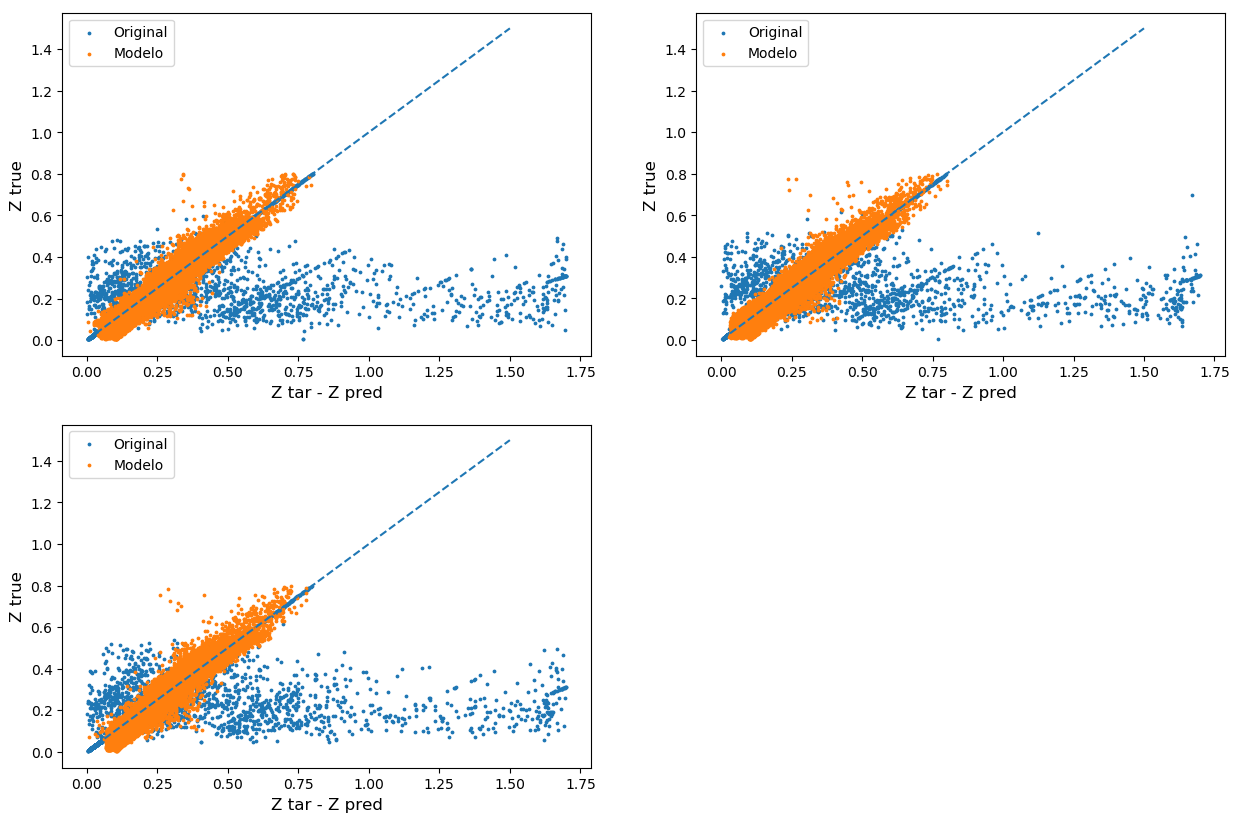
\includegraphics[width=1.0\linewidth]{TeX_files/Imagenes/svr-train}
	\caption{Results onthe training set after training the SVR model.}
	\label{fig:svr-train}
\end{figure}
The results on training set of the best models is shown in Figure \ref{fig:svr-train}. On training, the model shows good results by gathering the blue dots (original data)over the orange dots (the model results after applying it to the training data). The blue scatter is substantially diminished and the data is clustered along de TRUEZ = TARZ line, However, the data is not entirely over the line, but in a wide range. The result on the evaluation set for each model is show in Figure \ref{fig:svr-test}. 
\begin{figure}[th!]
	\centering
	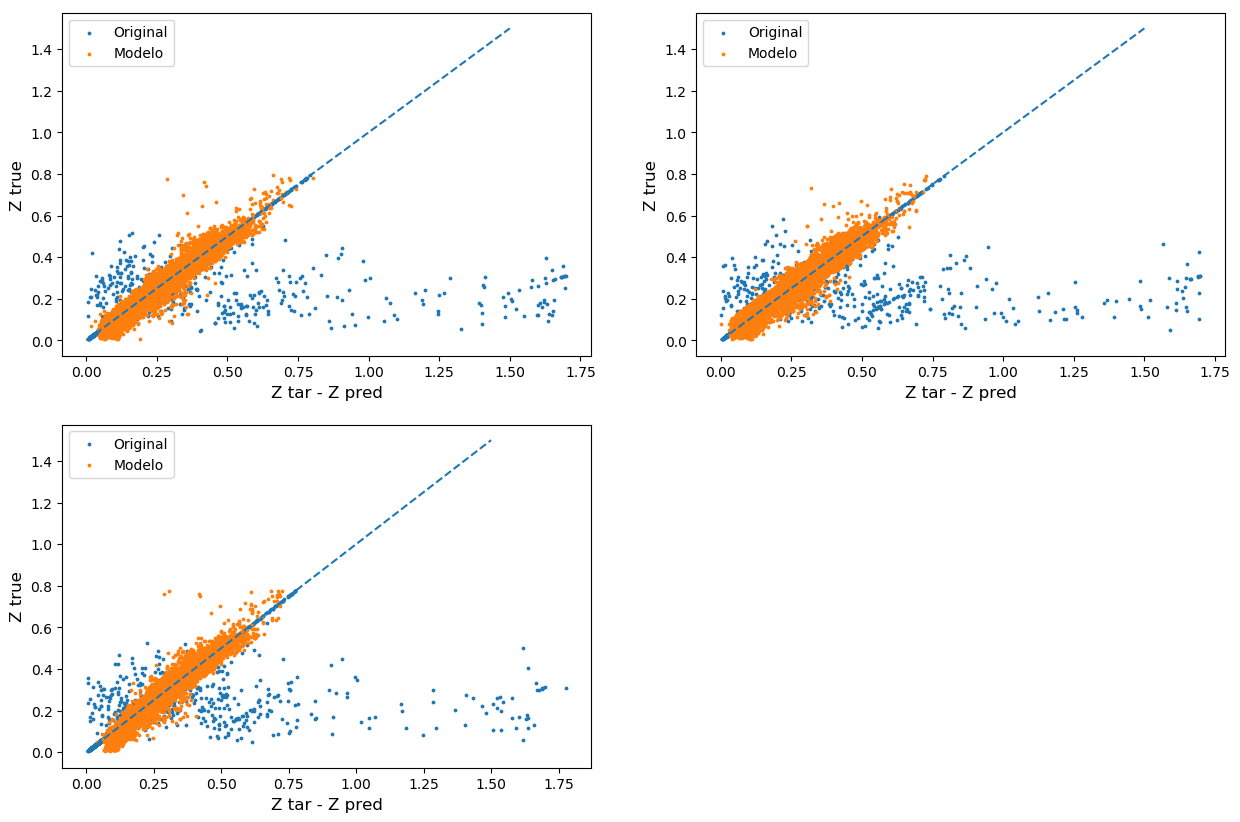
\includegraphics[width=1.0\linewidth]{TeX_files/Imagenes/svr-test}
	\caption{Results of each model on the development set.}
	\label{fig:svr-test}
\end{figure}
Figure \ref{fig:svr-test} shows how the model generalize to unseen data. The gathering capacity of the model to move the blue dots towards the TRUEZ = TARZ line present on the training set is also visible on the evaluation set, were the $r^2$ scores reaches 93\% only. 
\subsection{Kernel Ridge Regression (KRR) Model}

The grid-search and cross-validation on the train-development set use the $r^2$ measure to select the best parameters. 

\begin{verbatim}
--------------------------------------------------------------------------
Model 1:
Best parameters set found on development set:

{'alpha': 0.0001, 'gamma': 0.2, 'kernel': 'rbf'}

Grid scores on development set for r2:

0.986 (+/-0.002) for {'alpha': 0.001, 'gamma': 0.1, 'kernel': 'rbf'}
0.988 (+/-0.002) for {'alpha': 0.001, 'gamma': 0.2, 'kernel': 'rbf'}
0.987 (+/-0.002) for {'alpha': 0.0001, 'gamma': 0.1, 'kernel': 'rbf'}
0.989 (+/-0.002) for {'alpha': 0.0001, 'gamma': 0.2, 'kernel': 'rbf'}

r2 score computed on the full evaluation set:

0.990
--------------------------------------------------------------------------
Model 2:
Best parameters set found on development set:

{'alpha': 0.001, 'gamma': 0.2, 'kernel': 'rbf'}

Grid scores on development set for r2:

0.986 (+/-0.001) for {'alpha': 0.001, 'gamma': 0.1, 'kernel': 'rbf'}
0.988 (+/-0.002) for {'alpha': 0.001, 'gamma': 0.2, 'kernel': 'rbf'}
0.987 (+/-0.002) for {'alpha': 0.0001, 'gamma': 0.1, 'kernel': 'rbf'}
0.987 (+/-0.004) for {'alpha': 0.0001, 'gamma': 0.2, 'kernel': 'rbf'}

r2 score computed on the full evaluation set:

0.988
--------------------------------------------------------------------------
Model 3:
Best parameters set found on development set:

{'alpha': 0.001, 'gamma': 0.2, 'kernel': 'rbf'}

Grid scores on development set r2:

0.987 (+/-0.001) for {'alpha': 0.001, 'gamma': 0.1, 'kernel': 'rbf'}
0.988 (+/-0.002) for {'alpha': 0.001, 'gamma': 0.2, 'kernel': 'rbf'}
0.987 (+/-0.003) for {'alpha': 0.0001, 'gamma': 0.1, 'kernel': 'rbf'}
0.987 (+/-0.003) for {'alpha': 0.0001, 'gamma': 0.2, 'kernel': 'rbf'}

r2 score computed on the full evaluation set:

0.9899

\end{verbatim}
\begin{figure}[th!]
	\centering
	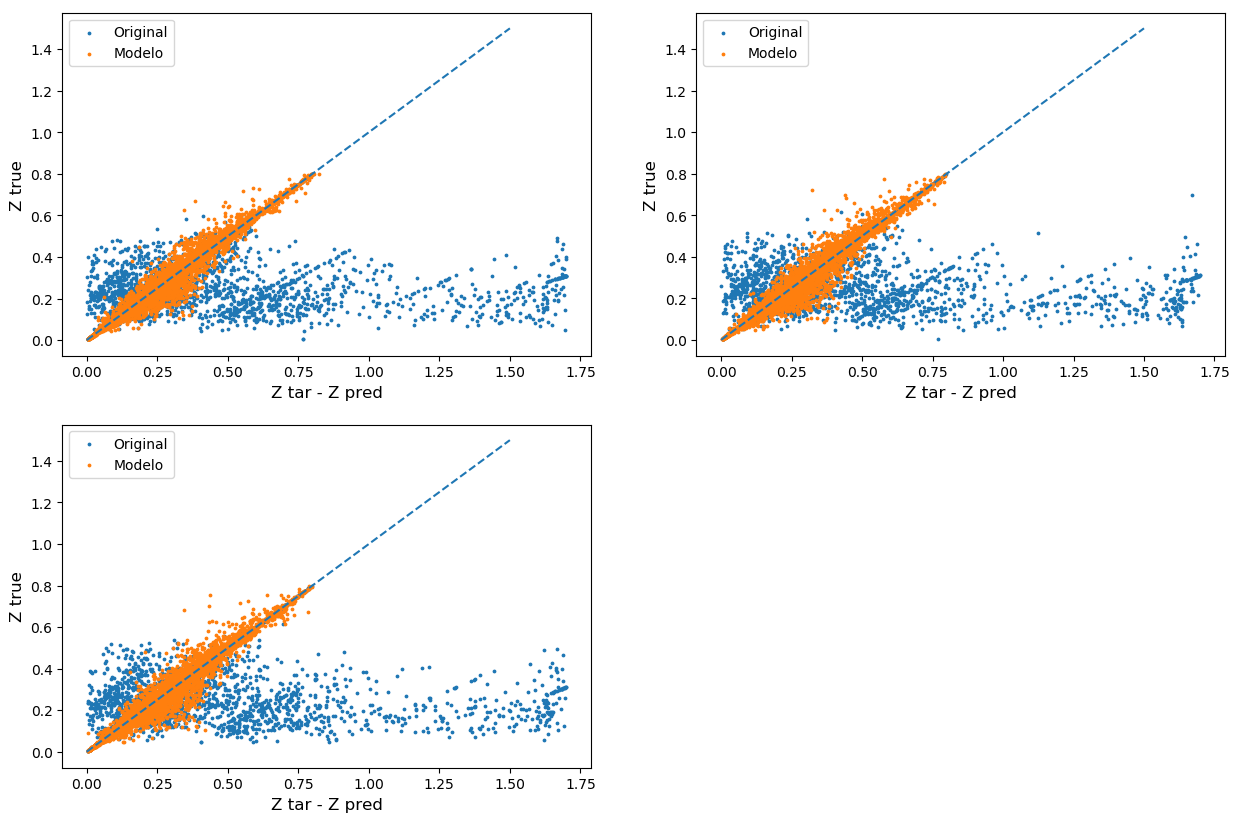
\includegraphics[width=1.0\linewidth]{TeX_files/Imagenes/krr-train}
	\caption{Results onthe training set after training the KRR model.}
	\label{fig:krr-train}
\end{figure}
The results on training set of the best models is shown in Figure \ref{fig:krr-train}. On training, the model shows better results than SVR by gathering the blue dots (original data)over the orange dots (the model results after applying it to the training data) on a tighter region. The blue scatter is substantially diminished and the data is clustered along de TRUEZ = TARZ line. The result on the evaluation set for each model is show in Figure \ref{fig:krr-test}. 
\begin{figure}[th!]
	\centering
	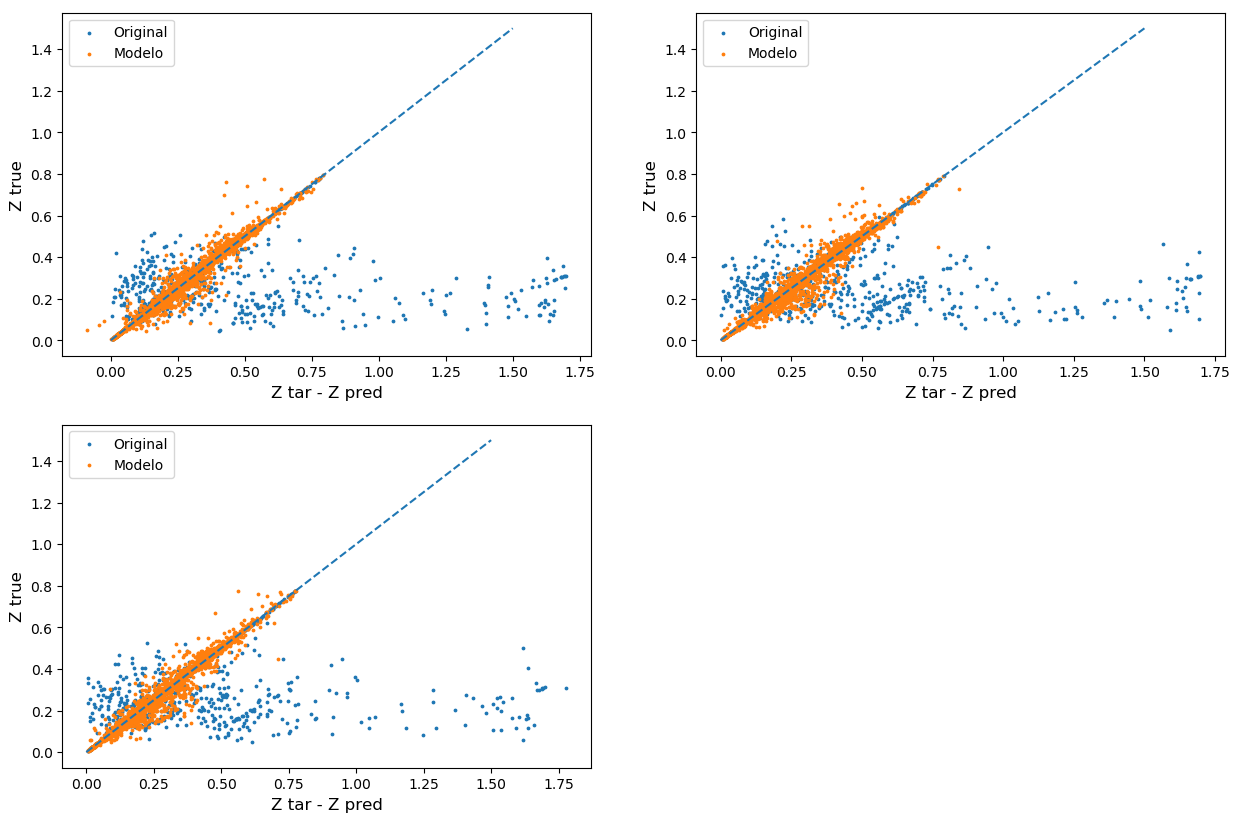
\includegraphics[width=1.0\linewidth]{TeX_files/Imagenes/krr-test}
	\caption{Results of each model on the development set.}
	\label{fig:krr-test}
\end{figure}
Figure \ref{fig:krr-test} shows how the model generalize to unseen data. The gathering capacity of the model to move the blue dots towards the TRUEZ = TARZ line present on the training set is also visible on the evaluation set, were the $r^2$ scores reaches 99\%, a more better result than that obtaining using SVR. 

\subsection{Model Ensemble}

The results from the KRR are much better than those of the SVR, also noting that the KRR model takes about half the time to train. Given that we have three different models to predict on the same dataset, we have to make this model to predict a single output. For this, we tried taking the maximum, the average or a weighted average of the model. 
\begin{figure}[h!]
	\centering
	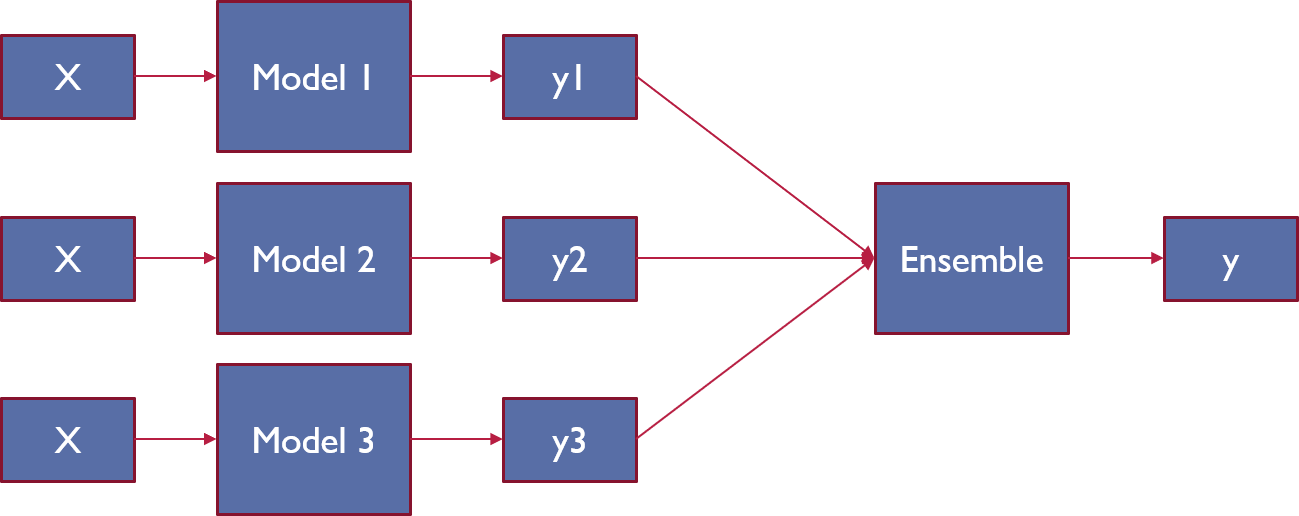
\includegraphics[width=1\linewidth]{TeX_files/Imagenes/ensemble_model}
	\caption{Graphic description of the ensemble model. It is formed based on the trained KRR models 1, 2 and 3.}
	\label{fig:ensemblemodel}
\end{figure}

Figure \ref{fig:ensemblemodel} shows this in a diagram, it is important to note that the ensemble is made over the \textbf{trained} models, that means that the parameters of the models are not re-learned in the ensemble. The only ensemble model that involves training, is the weighted average, where the weights are select by training a linear model. The results of the models on the \textbf{test} subset (unseen 25\%) are shown in Table \ref{table:test-result}. 

\begin{table}[h!]
	\centering
	\begin{tabular}{|c|c|}
		\hline 
		Model & $r^2$ \\ 
		\hline 
		Model 1 & 0.958 \\ 
		\hline 
		Model 2 & 0.956 \\ 
		\hline 
		Model 3 & 0.962 \\ 
		\hline 
		Model avg & 0.962 \\ 
		\hline 
		Model max & 0.949 \\ 
		\hline 
		Model w & 0.983 \\ 
		\hline 
	\end{tabular} 
    \caption{Results on the \textbf{test} set}
    \label{table:test-result}
\end{table}

Table \ref{table:test-result} shows that the weighted average of the three models is the best model in terms of accuracy, taking into account that this are the predictions of the models on the totally-unseen test data corresponding to the 25\% of the original BGS dataset. 
\section{Selección de modelo}

The class of models evaluated is that of kernels models, the complexity of both, the SVR and the KRR is very similar, however the KRR gave better results. This could be atributed to the lack of tuning of the $\epsilon$ parameter in SVR, due to the time of computation of SVR training. Smaller values of $\epsilon$, may result in a tighter region over the TRUEZ = TARZ line, therefore increasing the $r^2$. The weighted average model has at least 3 times more parameters that any model individually, its results are much better. Therefore, the best model, that keeps simplicity and very good results is the weighted average model. 

\section{Conclusions}

We evaluated two types of kernels method, the support vector regression (SVR) and the kernell ridge regression (KRR). The dataset was split in a training part (75\%) and a test part (25\%). Each model was trained tree times on subset of the training part of size 100.000, this subset were also subdivide in a 80-20 development - evaluation datasets for the application of grid search and cross validation. The KRR gave better results than the SVR, also, the three KRR models were ensemble as a weighted average, where the weights were found using a linear regressor. The ensemble average KRR model reached a $r^2$ of 0.98 on the test set. 
\chapter{Conclusions}
\label{Ch:conclusion}


%\chapter{Gravitational Collapse of non-perfect fluids}
As we have said before, the gravitational collapse of massive starts is one of the few observable scenarios where general relativity plays an important role, in contrast with many other astrophysical problems in which the Newtonian approximation is enough. It is therefore necessary to give a detailed description of this process adding more components to the original recipe of Oppenheimer and Snyder \cite{oppenheimer1939continued}. However it is valid to ask why should it be necessary to add more complication to the already complicated problem of gravitational collapse, such as the introduction of viscous, dissipative and radiating terms? The simple answer is that the gravitational collapse of stars \textit{is} a dissipative process and is can be proved as easily as follow: Let us make some rough estimates of the energy that consumes the gravitational collapse of a massive start to a 10 Km solar-mass-neutron star \textit{adiabatically} \cite{herrera2009relativistic}: The gravitational binding energy of a one solar mass of 10 Km is roughly given by
$$
E\approx -\frac{G M^2}{R} = -10^{53} erg
$$ 

Therefore, the collapse must release this amount of energy in order for the neutron star to form. Since we assume that the process occur adiabatically, then the internal energy, $E_{in}$ of the star must increase by that amount.  Now, assuming $E_{in} \approx kT$, where $k$ is the Boltzmann constant, then the temperature of such a system should rise the \textit{absurd} value of
\begin{equation}
\label{eq:TemperatureRiseAdiabCollapse}
	T\approx 10^{69} K,
\end{equation}
implying that after all is should radiate with luminosity of $10^{283} erg/s$. This would evaporate the star in less than a time of the order of $10^{-230}s$. Since all of these absurd values come from the original assumption that the whole process proceeds adiabatically, there must be some mechanism that allows the star to get rid of all the extra energy it has before collapsing\cite{herrera2009relativistic}.
\section{Equations for the interior space-time}
We assume a spherically symmetric distribution of fluid undergoing dissipation in the form of heat flow, free streaming radiation and shearing and bulk viscosity. The collapsing fluid is bounded by a surface $\Sigma$ and the viscosity dissipation terms are assumed to obey causal relations. In general comoving coordinates, the interior space-time is
\begin{equation}
	\label{eq:MetricInterior}
	ds^{2}_{-} = -A^2 (t, r)dt^2 + B^2 (t,r) dr^2 + (rC(t,r))^2d\Omega^2.
\end{equation}
Now we assume that the energy-momentum tensor of the collapsing matter is \cite{herrera2009dynamics}
\begin{equation}
	\label{eq:EnergyMomeTensorHerrera}
	T_{\alpha\beta} = (\rho + p + \Pi)U_{\alpha}U_{\beta} + (p + \Pi)g_{\alpha\beta} + q_{\alpha} U_{\beta} + q_{\beta} U_{\alpha} + \epsilon l_{\alpha}l_{\beta} + \pi_{\alpha\beta} .
\end{equation}
Note that this is the same energy-momentum tensor in \ref{eq:EnergyTensorNPF} with an additional term, the same from the source of the Vaidya metric \ref{eq:EMradiation}, where $\epsilon$ is the radiation density, and all the other variables are those defined in the previous chapters. These quantities satisfy
\begin{align}\nonumber
	U_{\alpha}U^{\alpha} &= -1, \qquad U^{\alpha}q_{\alpha} = 0 \qquad U^{\alpha}l_{\alpha} = -1 , \qquad l^{\alpha}l_{\alpha} = 0 \\\nonumber
	\pi_{\mu\nu}U^{\nu} &= 0, \qquad \pi_{[\mu\nu]} = 0, \qquad \tensor{\pi}{^{\alpha}_{\alpha}} = 0 \,\,\,\,\text{from this follow}\\\label{eq:Pidef}
	\pi_{0\alpha} &= 0 \qquad \tensor{\pi}{^{1}_1} = -2\tensor{\pi}{^{2}_2} = -2\tensor{\pi}{^{3}_3}.
\end{align}

Since we want a causal picture of dissipative variables, we cannot use the constitutive equation of standard irreversible thermodynamics \ref{eq:ConstitutiveEqEckart1}-\ref{eq:ConstitutiveEqEckart3}. This approach is discussed by many authors, including \cite{herrera2004dynamics} and \cite{pinheiro2008radiating}. The extended irreversible thermodynamic constitutive equations involve the kinematic tensors defined in \ref{eq:DefinitionKinematicTensors}, so the first part will be to write down this tensors in terms of the elements of the metric. First note that since the metric is comoving and the heat flow is radial:
\begin{equation}
	U^{\alpha} = A^{-1}\delta^{\alpha}_{0},\qquad q^{\alpha} = q(t,r) B^{-1}\delta^{\alpha}_1 ,\qquad l^{\alpha} = A^{-1}\delta^{\alpha}_{0} + B^{-1}\delta^{\alpha}_1, 
\end{equation}
also, from \ref{eq:Pidef} we can write
\begin{equation}
	\label{eq:Pidef2}
	\pi_{\alpha\beta} = \Omega(\chi_{\alpha}\chi_{\beta} - \frac{1}{3}h_{\alpha\beta}) ,
\end{equation}
where $\chi^{\alpha}$ is a unit four vector along the radial direction and $\Omega = 3/2\pi^{1}_{1}$. Next we compute the non vanishing components of the shear tensor defined in \ref{eq:DefinitionKinematicTensors},
\begin{equation}
	\sigma_{11} = \frac{2}{3}B^2 \sigma ,\qquad \sigma_{22} = \frac{\sigma_{33}}{\sin ^2 \theta} = -\frac{1}{3} (Cr)^2 \sigma ,
\end{equation}
where
\begin{equation}
	\sigma = \frac{1}{A}\left(\frac{\dot{B}}{B} - \frac{\dot{C}}{C}\right) = \left( \frac{3}{2} \sigma_{\alpha\beta}\sigma^{\alpha\beta} \right)^{1/2}.
\end{equation}
The 4-acceleration and the expansion, given as well by \ref{eq:DefinitionKinematicTensors} are:
\begin{equation}
	a_1 = \frac{A'}{A} \qquad \Theta = \frac{1}{A} \left( \frac{\dot{B}}{B} + 2 \frac{\dot{C}}{C} \right),
\end{equation}
the dot stands for differentiation with respect to $t$, and the prime stands for $r$ differentiation. Now we proceed to the Einstein field equations given by
\begin{equation}
	G_{\alpha\beta}^{-} = 8\pi T^{-}_{\alpha\beta} .
\end{equation}
From section \ref{sec:ComovingCoordinates} we know that the non vanishing components of the Einstein tensor are
\begin{equation}
	G_{00}^{-}, \qquad G_{11}^{-} ,\qquad G_{22}^{-} ,\qquad G_{33}^{-} = \sin ^2 \theta G_{22}^{-}, \qquad G_{01}^{-} .
\end{equation}
According to \ref{eq:EinsteinTensorComovingCH}. The corresponding components of the energy-momentum tensor are:
\begin{align}
	8\pi T_{00}^{-} &= 8\pi (\rho + \epsilon)A^2, \\
	8\pi T_{11}^{-} &= 8\pi \left[p + \Pi + \epsilon + \frac{2}{3}\Omega \right],\\
	8\pi T_{22}^{-} &= 8\pi \left[p + \Pi - \frac{\Omega}{3}\right](Cr)^2 ,\\
	8\pi T_{01}^{-} &= -8\pi(q + \epsilon) AB.
\end{align}

\section{Exterior spacetime}
The metric outside the collapsing star correspond to the metric of a spherically radiating source, this means, a Vaidya metric as shown in section \ref{sec:VaidyaMetric}. The line element is
\begin{equation}
	\label{eq:VaidyaMetricB}
	ds^{2}_{+} = - \left(1 - \frac{2m(\nu)}{\textbf{r}}\right)d\nu^2 - 2 d\textbf{r}d\nu + \textbf{r}^2d\Omega^2.
\end{equation}
We have to apply the two junction conditions \ref{eq:FirstJunctCon} and \ref{eq:SecondJunctCond},
\begin{align}
	(ds^{2}_{-})_{\Sigma} &= (ds^{2}_{+})_{\Sigma}, \\
	K_{ab}^{-} &= K_{ab}^{+}.
\end{align}
We choose on $\Sigma$ the standard intrinsic coordinates $\tau, \theta, \phi$ and proceed to compute the induced metric, and obtain
\begin{align}
\label{eq:FirstJcond}
	A(t, r_{\Sigma})\frac{dt}{d\tau} &= 1,\\\nonumber
	C(r_{\Sigma}, t) r_{\Sigma} &= \textbf{r}_{\Sigma}(\nu) ,\\\nonumber
	\left(\frac{d\nu}{d\tau}\right)^{-2}_{\Sigma} &= \left(1 - \frac{2m(\nu)}{\textbf{r}} + 2\frac{d\textbf{r}}{d\nu}\right)_{\Sigma}.
\end{align}
Now we proceed with the computation of the second fundamental form: In the interior coordinates, $\Sigma$ is defined by $\Phi = r - r_{\Sigma} = 0$, the corresponding normal vector is calculated as $\partial_{\alpha}\Phi$ and normalized:
\begin{equation}
\label{eq:NormalToSigmaIN}
	n_{\alpha}^{-} = \{0, B(r_{\Sigma},t), 0,0\}
\end{equation} 
Now, the non-vanishing components of the extrinsic curvature given by \ref{eq:ExtrinsicCurv} are
\begin{align}
	\label{eq:ExtrinsicCurvInt1}
	K_{\tau\tau}^{-} &= - \left[\left(\frac{dt}{d\tau}\right)^2\frac{AA'}{B}\right]_{\Sigma}, \\	\label{eq:ExtrinsicCurvInt2}
	K_{\theta\theta}^{-} &= \left(\frac{(rC' +C)rC}{B}\right)_{\Sigma},\\
	K_{\phi\phi}^{-} &=  K_{\theta\theta}^{-}\sin^2 \theta.
\end{align}
In the exterior, the equation of $\Sigma$ is given by $\textbf{r} - \textbf{r}_{\Sigma}(\nu)=0$ therefore, $\partial_\alpha \Phi = \{ -d\textbf{r}_{\Sigma} / d\nu, 1, 0, 0\}$ and
\begin{equation}
	n_{\alpha}^{+} = \left(1 - \frac{2m}{\textbf{r}} + 2 \frac{d\textbf{r}}{d\nu}\right)_{\Sigma}^{1/2} \left\{ -d\textbf{r} / d\nu, 1, 0, 0\right\}_{\Sigma}.
\end{equation}
The non vanishing components of the extrinsic curvature are
\begin{align}
	\label{eq:ExtrinsicCurvExt1}
		K_{\tau\tau}^{+} &= \left[\frac{d^2\nu}{d\tau^2} \left(\frac{d\nu}{d\tau}\right)^{-1} - \left(\frac{d\nu}{d\tau}\right)\frac{m}{\textbf{r}} \right]_{\Sigma}, \\\label{eq:ExtrinsicCurvExt2}
			K_{\theta\theta}^{+} &= \left[\left(\frac{d\nu}{d\tau}\right)\left(1 - \frac{2m}{\textbf{r}}\right)\textbf{r} + \frac{d\textbf{r}}{d\tau}\textbf{r}\right]_{\Sigma},\\\label{eq:ExtrinsicCurvExt3}
		K_{\phi\phi}^{+} &=  K_{\theta\theta}^{+}\sin^2 \theta	.		
\end{align}

From \ref{eq:ExtrinsicCurvExt2} and \ref{eq:ExtrinsicCurvInt2} we get
\begin{equation}
 \left[\left(\frac{d\nu}{d\tau}\right)\left(1 - \frac{2m}{\textbf{r}}\right)\textbf{r} + \frac{d\textbf{r}}{d\tau}\textbf{r}\right]_{\Sigma} =  \left(\frac{(rC' +C)rC}{B}\right)_{\Sigma}.
\end{equation}
With the help of \ref{eq:FirstJcond} we can rewrite this as our first result:
\begin{equation}
\label{eq:VaidyaMass}
	m = \frac{Cr}{2}\left\{ \left(\frac{r\dot{C}}{A}\right)^2 - \left[\frac{(Cr)^2}{B}\right]^2 + 1\right\}.
\end{equation} 
This is quite interesting since the rhs correspond to the same mass defined by Misner and Sharp in \cite{misner1964relativistic}. From the equality of the remaining independent component of the extrinsic curvature, and again \ref{eq:FirstJcond}, we get \cite{pinheiro2008radiating}\cite{herrera2009dynamics}
\begin{align}\nonumber
	2 \frac{\dot{C}'}{C} &+ 2 \frac{\dot{C}}{Cr} - 2\frac{\dot{B}C'}{BC} - 2\frac{\dot{B}}{Br} - 2\frac{A'\dot{C}}{AC} + \\
	&= \frac{B}{A} \left[2\frac{\ddot{C}}{C} -2\frac{\dot{C}\dot{A}}{CA} + \left(\frac{A}{Cr}\right)^2 + \left(\frac{\dot{C}}{C}\right)^2 - \left(\frac{A}{B}\right)^2 \left(\frac{C'}{C} + \frac{1}{r}\right)\left(\frac{C'}{C} + \frac{1}{r} + 2 \frac{A'}{A}\right)\right]_{\Sigma} = 0,
\end{align}
comparing this with $G_{11}$ and $G_{01} $ and its corresponding energy-momentum counterparts, we can rewrite the last equation in a very compact way
\begin{equation}
	\label{eq:SecondJcond}
	\left(p + \Pi + \frac{2}{3}\Omega\right)_{\Sigma} = q_{\Sigma},
\end{equation}
then, the matching of \ref{eq:MetricInterior} and \ref{eq:VaidyaMetricB} at $\Sigma$ implies \ref{eq:VaidyaMass} and \ref{eq:SecondJcond}. 

\section{Hydrodynamic Equations}
The hydrodynamical equations are the same as \ref{eq:EnergyEquationNPF} and \ref{eq:MomentumEquationNPF}, but with an extra term that comes from the radiation density. In terms of the kinematic tensor that we found before this equations are:
\begin{align}
	\label{eq:EnergyConserNPFHERR}
	U_{\alpha} \tensor{T}{^{-\alpha\beta}_{;\alpha}} &= -\frac{1}{A}(\dot{\rho} + \dot{\epsilon}) - \frac{1}{B}(q' + \epsilon') - 2(q+\epsilon) \frac{(ACr)'}{ABCr} - \frac{2\dot{C}}{AC}\left(\rho + p + \Pi + \epsilon - \Omega/3\right) \\\nonumber
	&- \frac{\dot{B}}{AB} \left(\rho + p + \Pi + 2\epsilon + \frac{2}{3} \Omega \right) = 0,
\end{align}
and the momentum equation 
\begin{align}
\label{eq:MomentumConseNPFHERR}
	\tensor{T}{_{\nu}^{-\mu\nu}}\chi_{\mu} & = \frac{1}{A} (\dot{q} + \dot{\epsilon}) +  \frac{2\dot{(BC)}}{BC} (q+ \epsilon) + \frac{1}{B}\left(p' + \Pi' + \epsilon' + \frac{2}{3}\Omega'\right) \\\nonumber &+ \frac{A'}{BA} \left(\rho + p + \Pi + 2\epsilon + \frac{2}{3}\Omega\right) + \frac{2(Cr)'}{BCr} (+\epsilon + \Omega) = 0.
\end{align}

Now, to study the dynamical properties of the system we introduce the proper time derivative $D_T$ and the proper radial derivative $D_R$ \cite{herrera2009dynamics}\cite{misner1964relativistic} given by
\begin{equation}
	D_T = \frac{1}{A}\frac{\partial}{\partial t} \qquad D_R = \frac{1}{R'} \frac{\partial}{\partial r},
\end{equation}
where $R = Cr$, defines the proper radius of a spherical surface inside $\Sigma$. Using this two derivatives we can define the velocity of the collapsing fluid in shell of radius r as $U = D_T R = rD_T C $. Note that for the case of collapse $U<0$. With this we can rewrite the Vaidya mass in \ref{eq:VaidyaMass} in a more practical way
\begin{equation}
	E \equiv \frac{R'}{B} = \left[1 + U^2 - \frac{2m(t, r)}{R}\right]^{1/2}.
\end{equation}
Next, after some algebra, the Einstein equations lead to the following important equations:
\begin{equation}
\label{eq:Dtdm}
	D_T m = -4\pi R^2\left[\left(p + \Pi + \epsilon + \frac{2}{3}\Omega\right)U + (q+\epsilon)E\right] ,
\end{equation}
and
\begin{equation}
\label{eq:Drdm}
	D_R m = 4\pi R^2 \left[\rho + \epsilon + (q + \epsilon)\frac{U}{E}\right] .
\end{equation}
This two equations describe the behavior of the mass of the star temporally and spatially.  The equation \ref{eq:Dtdm} describes the rate of variation of the total energy inside a surface radius R. In the case of collapse, since U is negative, the first term on the rhs of \ref{eq:Dtdm}, $\left(p + \Pi + \epsilon + 2\Omega/3\right)U$ is negative, and therefor, since there is a minus sign in front, this terms increases the energy (mass) of the system due to the rate of work that is done by the effective pressure $p + \Pi + 2\Omega/3$ and the radiation pressure $\epsilon$. The other term, since $(q+\epsilon)E$ is the matter energy leaving the surface. Therefore, the rate of change of the total energy (that is the Vaidya mass) is the sum of a 'thermodynamic' or 'hydrodynamic' work don on the system a the matter energy leaving the system. The equation \ref{eq:Drdm} shows how the total energy varies in different shells of different radius, the first two terms $\rho + \epsilon$ are the the spatial distribution of matter, energy density of the fluid element plus the null fluid (radiation).  The other term measures the outflow of heat and radiation. The acceleration of the collapsing surface $D_T U$ can be computed from the (11) component of the Einstein equation, after that, we use it to write the conservation of momentum \ref{eq:MomentumConseNPFHERR} in therms only of the thermodynamic fluxes, we get
\begin{align}
	\label{eq:ConserMomentumFluxes}
	\left(\rho + p + \Pi + 2\epsilon + \frac{2}{3}\Omega\right)D_T U &= \left(\rho + p + \Pi + 2\epsilon + \frac{2}{3}\Omega\right)\left[\frac{m}{R^2} + 4\pi R\left(\rho + p + \Pi + \epsilon + \frac{2}{3}\Omega\right) \right] \\\nonumber
	&-E^2 \left[D_R\left(\rho + p + \Pi + \epsilon + \frac{2}{3}\Omega\right) + \frac{2}{R}(\epsilon + \Omega)\right]\\\nonumber &- \left[D_T q + D_T \epsilon + 4(q+\epsilon)\frac{U}{R} + 2(q+\epsilon)\sigma \right].
\end{align}
This equation has the 'Newtonian' form 
$$
\text{Force}\, = \,\text{Mass density}\,\, \times \,\,\text{Acceleration}
$$
The factor in round brackets represent the effective inertial mass. The first term with square brackets in the r.h.s. of \ref{eq:ConserMomentumFluxes} represent the gravitational forces, it shows that  the gravitational force acting on a particle has a Newtonian part with $m$ and a purely relativistic gravitational contribution due to $p, \epsilon, \Pi$ and $\Omega$. Also, this term shows how dissipation affects the 'active' gravitational mass term. In the second square bracket, the hydrodynamical force, are two separate contributions, the first one is the gradient of the total effective pressure, which includes the radiation pressure and the influence of shear and bulk viscosity, this is the term that counteracts the collapse, and the second contribution comes from the local anisotropy of pressure induced by the radiation pressure and shear viscosity\cite{herrera2009dynamics} \cite{herrera2004dynamics}. The las term in square brackets contains the specific contribution of dissipation to the dynamics of the system, $q + \epsilon$ is positive, meaning that the outflow of heat and radiation decreases the total energy inside the collapsing sphere, reducing the rate of collapse. We still have no information about the dissipative terms in the energy momentum tensor, we need some equations to see how this coefficient behave, this equation are called transport equations, and are precisely the same constitutive equation derived in the previous chapter.

\section{Coupling the transport equations}

We already know the constitutive equation in the Eckart frame of the extended irreversible thermodynamics. This equations (\ref{eq:PhenomEq1}-\ref{eq:PhenomEq3}) relate the three thermodynamic fluxes with a series of parameters and coupling constant that ended up grouping in 'relaxation times' $\tau_0, \tau_1, \tau_2$. We re rearrange eq. \ref{eq:PhenomEq1}-\ref{eq:PhenomEq3} (and use the definitions of tensor quantities in terms of metric components) to obtain dynamic equations for the three fluxes, 
\begin{equation}
\label{eq:Transport1}
	\tau_0 \dot{\Pi} = -\left(\zeta + \frac{\tau_0}{2}\Pi\right)A\Theta + \frac{A}{B} \alpha_0 \zeta \left[q' + q\left(\frac{A'}{A} + \frac{1(Cr)'}{Cr}\right)\right] - \Pi\left[\frac{\zeta T}{2}\dot{\left(\frac{\tau_0}{\zeta T}\right)} + A\right],
\end{equation} 
\begin{align}
	\label{eq:Transport2}
	\tau_1 \dot{q} &= -\frac{A}{B}\kappa \left\{ T' \left(1 + \alpha_0 \Pi + \frac{2}{3} \alpha_1 \Omega\right) + T\left[\frac{A'}{A} - \alpha_0 \Pi' - \frac{2}{3} \alpha_1 \left(\Omega' + \Omega\left(\frac{A'}{A} + 3\frac{(rC)'}{rc}\right)\right)\right]  \right\} \\\nonumber 
	&- q\left[\frac{\kappa T^2}{2}\dot{\left(\frac{\tau_1}{\kappa T^2} \right)} + \frac{\tau_1}{2}A\Theta + A\right],
\end{align}

\begin{equation}
	\label{eq:Transport3}
	\tau_2 \dot{\Omega} = -2\eta A\sigma + 2 \eta\alpha_1 \frac{A}{B} \left(q' - q\frac{(rC)'}{rC}\right) - \Omega \left[\eta T \dot{\left(\frac{\tau_2}{2\eta T}\right)} + \frac{\tau_2}{2}A\Theta + A\right].
\end{equation}
Now we have to couple this equations with equation \ref{eq:ConserMomentumFluxes}, in order to bring out the effects of dissipation on the dynamics of the collapsing sphere. We replace \ref{eq:Transport1} and \ref{eq:Transport2} in \ref{eq:ConserMomentumFluxes} and obtain \cite{herrera2009dynamics}
\begin{align}
\nonumber
	&\left(\rho + p + \Pi + 2\epsilon + \frac{2}{3}\Omega\right)(1 - \Gamma + \Delta) D_T U = (1-\Gamma + \Delta)F_{g} + F_{H} \\\nonumber
	&\frac{\kappa E^2}{\tau_1} \left\{ D_R T\left(1 + \alpha_0\Pi + \frac{2}{3}\alpha_1 \Omega\right)- T\left[\alpha_0 D_R\Pi + \frac{2}{3}\alpha_1\left(D_R \Omega + \frac{3}{R}\Omega\right)\right] \right\} \\\nonumber
	&-E^2\left(\rho + p + \Pi + 2 \epsilon + \frac{2}{3} \Omega\right)\Delta\left(\frac{D_R q}{q} + \frac{2q}{R}\right)\\\nonumber
	&+ E\left[\frac{\kappa T^2 q}{2\tau_1}D_T \left(\frac{\tau_1}{\kappa T^2}\right) - D_T \epsilon\right] + E\left[\frac{q}{\tau_1} + 2(q+\epsilon)\frac{U}{R}\right] \\
	\label{eq:MasterEquationTesis}
	&+E\frac{\Delta}{\alpha_0 \zeta q} \left(\rho + p + \Pi + 2\epsilon + \frac{2}{3} \Omega\right)\left\{ \left[1 + \frac{\zeta T}{2}D_T \left(\frac{\tau_0}{\zeta T}\right) \right]\Pi + \tau_0 D_T \Pi \right\}
\end{align}

In this gigantic master equation several definitions where made:
\begin{align}
	F_g &= -\left(\rho + p + \Pi + 2\epsilon + \frac{2}{3}\Omega\right)\left[m + 4\pi \left(p+\Pi + \epsilon + \frac{2}{3}\Omega\right)R^3\right]\frac{1}{R^2} \\
	F_H &= -E^2 \left[D_R\left(p + \Pi + \epsilon + \frac{2}{3}\Omega \right) + 2(\epsilon + \Omega)\frac{1}{R}\right] \\
	\Lambda &=  \frac{\kappa T}{\tau_1}\left(\rho + p + \Pi + 2\epsilon + \frac{2}{3}\Omega \right)^{-1} \left(1 - \frac{2}{3}\alpha_1 \Omega\right) \\
	\Delta &= \alpha_0 \zeta q\left(\rho + p + \Pi + 2\epsilon + \frac{2}{3}\Omega\right)^{-1}\left(\frac{3q + a \epsilon}{2\zeta + \tau_0 \Pi}\right)
\end{align}

This means that once transport equations have been taking into account, the internal energy density and the effective inertial mass appear diminished by the same factor $1 - \Lambda + \Delta$. Note also that as $\Lambda - \Delta = \nu $ tends to 1, the effective inertial mass density of the fluid element tends to zero, but since $F_g$ is also multiplied by the same factor we see that the effective gravitational attraction on any fluid element decreases by the same factor, which of course is to be expected from the equivalence principle. Also note that $F_H$ seams to be in principle independent of this factor. It could be the case in which a collapsing star evolves in such a way, that the value of $\nu$ keeps approaching 1, as this happens, the decreasing of gravitational force term would eventually lead to a change of sign in the acceleration. Since this would happen for small values of the effective inertial mas density, that would imply a strong bouncing of the sphere, as the described by \cite{may1966hydrodynamic} in the case of the collapse of a perfect fluid. This kind of behavior could be accomplished in the formation of a neutron star in a supernova explosion \cite{herrera2004dynamics}.

\section{Conclusions}

The important remarks on the equation have already been made, however, it is important to make something clear. The dissipative variables have a major effect on the internal energy and the effective inertial mass, this effect could result in bouncing or a stagnation of the collapse depending on the value of the coefficients defined. Nevertheless, the role that this effect might play in the outcome of gravitational collapse will critically depend on the specific numerical values of those quantities, and such estimations require the conditions of a real astrophysical event. Therefore, with this presenting here we wanted to show how the dissipative and coupling coefficients enter in the dynamical equations and why their effect could be important and should be taken into account for numerical simulation. The parameter $\nu$ could reach unity in non very exotic systems, such as the formation of a neutrino star and in a supernova explosion. Indeed, at last stages of massive star evolution, the decreasing of the opacity of the fluid, from high values preventing the propagation of photons and neutrinos, to smaller values, gives rise to radiative heat conduction. And under this conditions, both $\kappa$ and $T$ could be sufficiently large as to imply a substantial increase of $\nu$ \cite{herrera2009relativistic}. 

It could be interesting also to study the behavior of these equation using computational techniques, in the study of a particular astrophysical event. The nature of the fluid (its equation of state) and the initial conditions of the scenario can be investigated in order to propose some reasonable values for the relaxation times and see how the process evolves. This could then be compared with results in non-causal theories and experiments to see the relevance of the causal theory of dissipation and its tangible effects on the dynamics of the collapse.








\backmatter
% bibliography, glossary and index would go here.
\bibliographystyle{ieeetr}
\bibliography{referencias}

\end{document}